\documentclass[14pt,letterpaper]{article}
\usepackage[margin=2cm,includefoot]{geometry}
\usepackage[spanish]{babel}
\usepackage[utf8]{inputenc}

\usepackage[colorlinks = true,
            linkcolor = blue,
            urlcolor  = blue,
            citecolor = blue,
            anchorcolor = blue]{hyperref}

 
 
\usepackage{amsmath}
\usepackage{graphicx}
\usepackage{listings}
\usepackage{array}
\usepackage{tikz-qtree}
\usepackage{lscape}

\graphicspath{ {images/} }




\title{Tarea 1}
\author{}
\date{}

\begin{document}

\ttfamily
\maketitle
\rmfamily
\begin{enumerate}
\item {\bf Instrucciones.}
  
  \item {\bf Agentes.}

    A continuación se muestra nuestro análisis de
    cada caso de acuerdo a nuestra solución:
    
    \begin{itemize}
    \item Agente Aleatorio.

      Este es el único que es no-determinista, pues
      al funcionar mediante la función {\it choice}
      el comportamiento no puede ser anticipado o
      que siempre se repita.

      En una ejecución que hicimos sucede los siguiente:

      %% Imagen
      \begin{centering}
        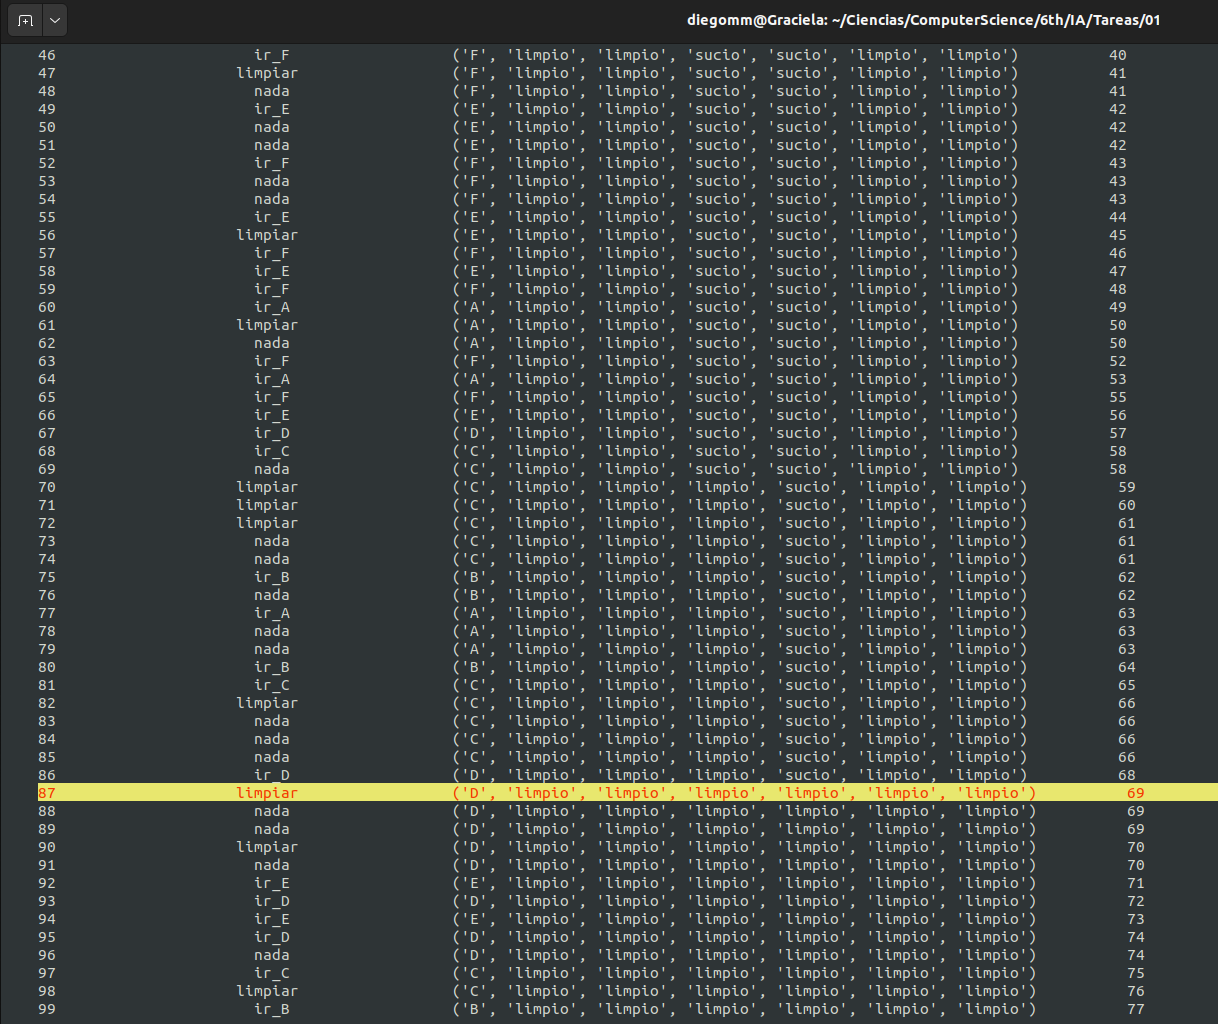
\includegraphics[scale=.3]{aleatorio}
      \end{centering}
      
      Nuestro agente termina de limpiar
      los seis cuartos en la iteración/decisión 87
      y con un costo de 69 y terminando las cien
      iteraciones con un costo de 77.

      Las cien iteraciones pueden o no ser suficientes
      para limpiar los sesis cuartos, así que no podriamos decir
      que funciona de una manera optima.
      \newpage
    \item Agente reactivo Simple.

      Al igual que el siguiente agente este es determinista
      y lo que hace es comenzar en A, para el cuarto en el que se encuentre
      si el estado es sucio procede a limpiar y si no no importa el cuarto
      en la que se encuentre se mueve haciendo un ``circulo'' hacia la derecha,
      es decir siguiendo el recorrido:

      $$ A\rightarrow B \rightarrow C \rightarrow D \rightarrow E \rightarrow F \rightarrow A ...$$

      %% Imagen
      \begin{centering}
        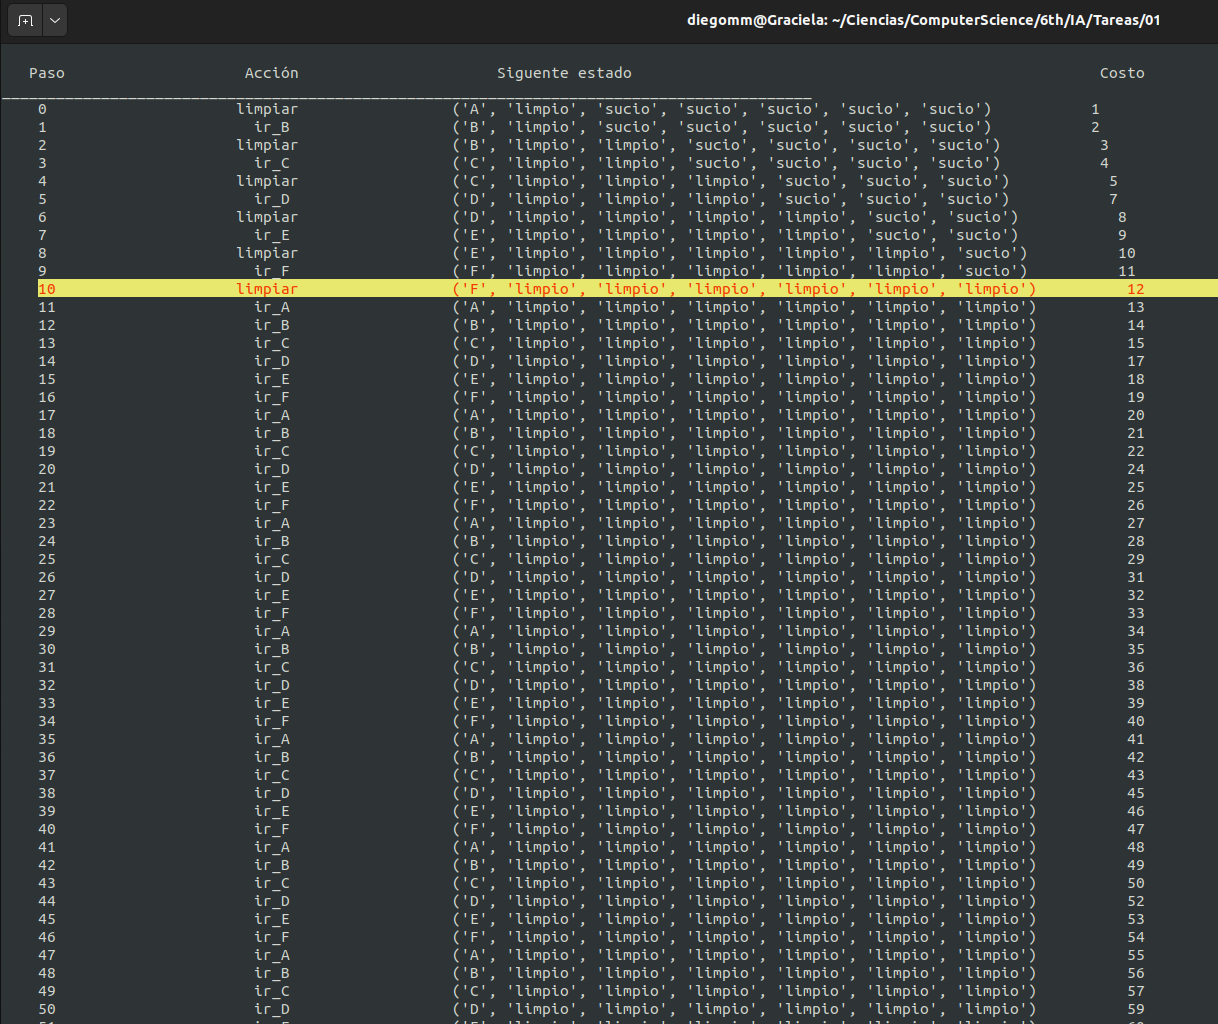
\includegraphics[scale=.3]{simple}
      \end{centering}

      Vemos que para la decima iteración los seis cuartos se encuentran limpios con un costo
      de 12,  pero al ser simple y solo reaccionar a lo que se encuentra nunca para
      su recorrido y lo perpetua durante las cien iteraciones. Terminando
      con un costo de 116. Pareciera ser más optimo en el tiempo en el que
      limpia pero como nunca descansa el costo al final {\it puede} ser peor
      que el del aleatorio.     
      \newpage      
    \item Agente reactivo con Modelo.

      Para este solo faltaba optimizar lo restante del agente anterior,
      que es hacer que nuestro robot se pare en cuanto haya limpiado todos los cuartos.
      En la vida real quiza habria que programarlo para escanear los cuartos en busca de
      algún sucio o poder informarle mediante una aplicación que cierto cuarto
      se ensució.

      %% Imagen
      \begin{centering}
        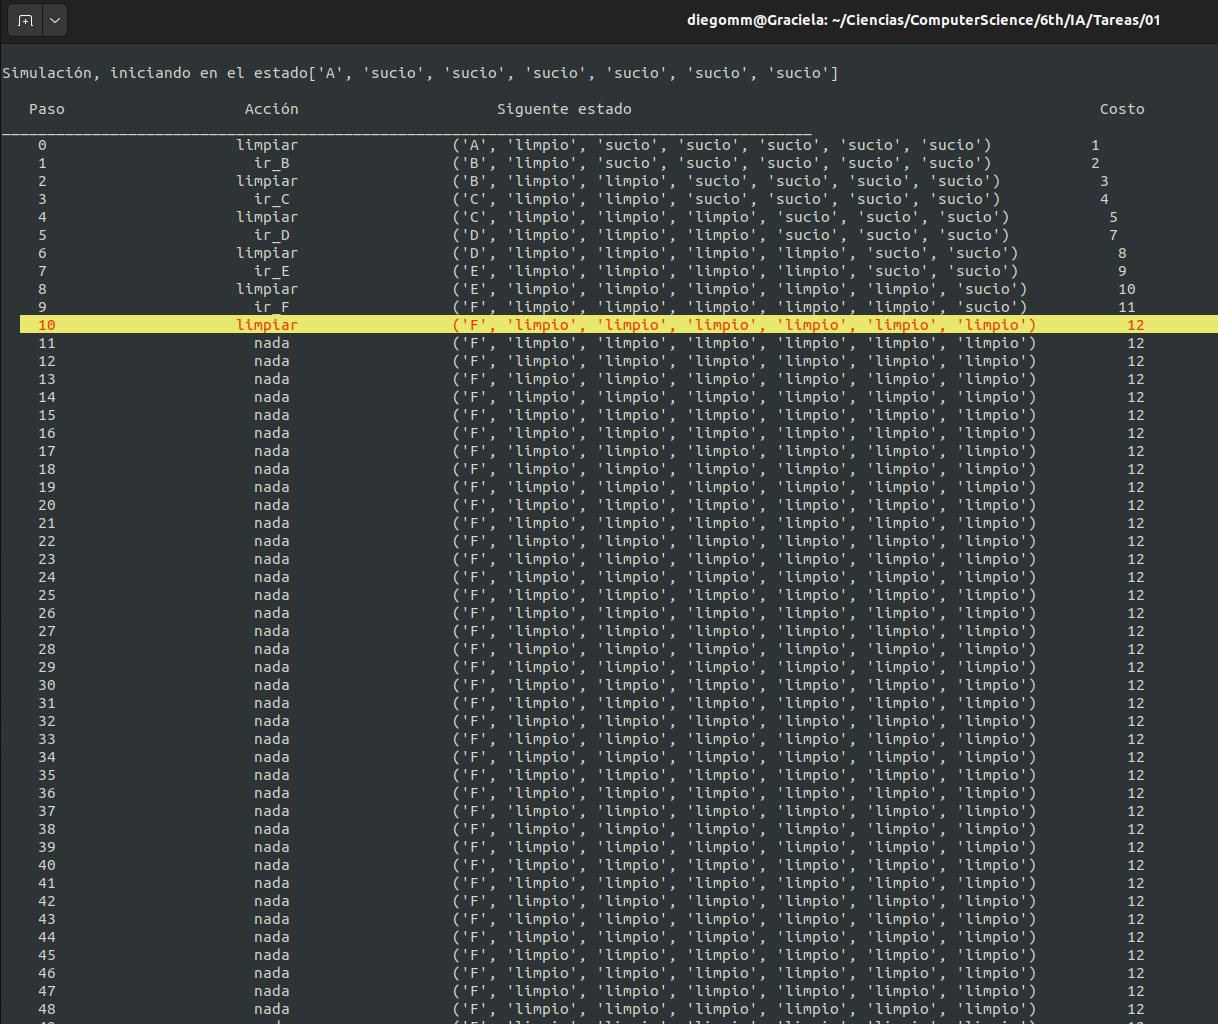
\includegraphics[scale=.3]{modelo}
      \end{centering}
      
      Tambíen termina en la decima iteración, pero de ahí en adelante ya no
      hace nada es decir no genera costo.
    \end{itemize}
    
  \item {\bf Búsqueda Ciega.}

    La implementación se encuentra en el archivo {\it tarea\_1.py} y al
    ejecutarlo se corre sobre la gráfica solicitado. El resultado se muestra
    en la salida standard despúes de la sección de los agentes.

    Nuestra ejecución devuelve el siguiente topological sort:

      %% Imagen
      \begin{centering}
        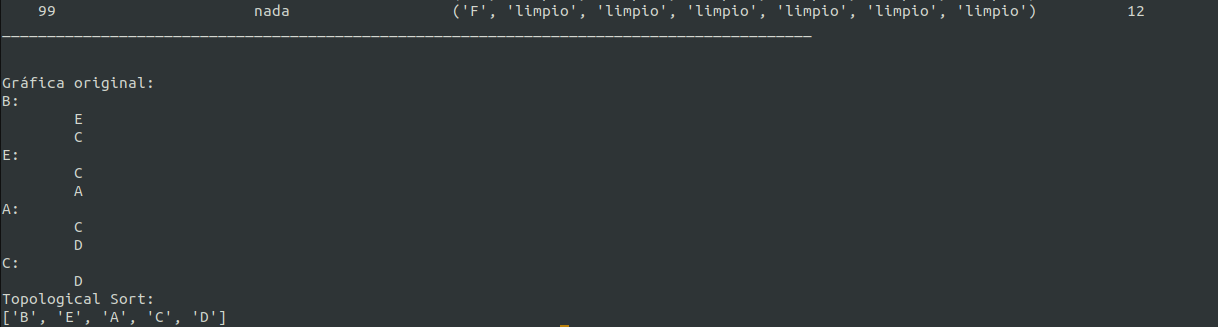
\includegraphics[scale=.3]{topological_sort}
      \end{centering}

      Que cumple con la definicion de orden topologico.
      \newpage
    \item {\bf Búsqueda Informada.}

      \begin{enumerate}
      \item Utilizando la imagén que se muestra a continuación:\href{https://www.gob.mx/cms/uploads/attachment/file/559748/SFM_2020_ESQUEMATICO_.pdf}{Obtenida de gob.mx}

      \begin{centering}
        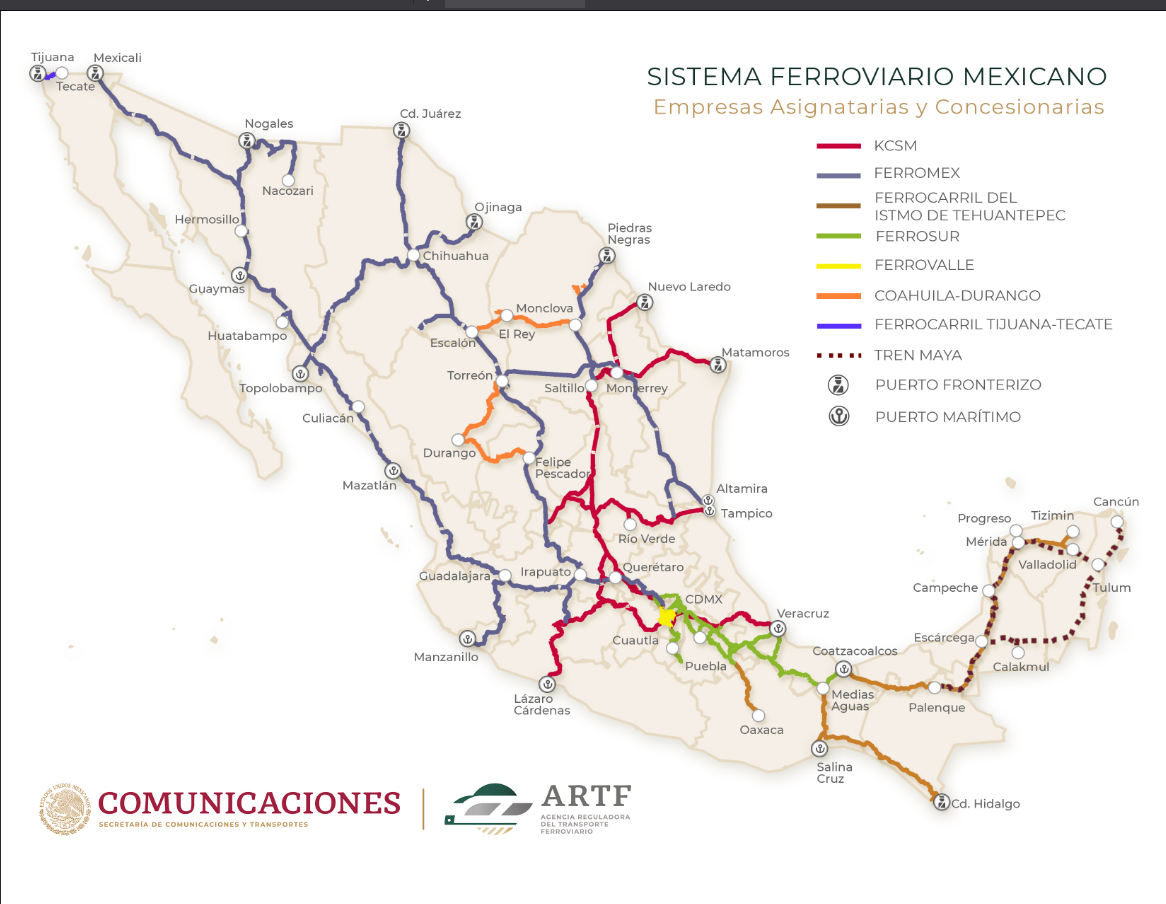
\includegraphics[scale=.3]{ferroviario}
      \end{centering}

      Es que nos queda claro que ciudades(las que intersectan dos sistemas distintos) son las
      que nos van a auxiliar. Con base en eso y una busqueda tenemos la siguiente tabla
      de distancias:

      \begin{table}[h]
        \centering
        \begin{tabular}{|c|c|c|}
          \hline
              {\bf Ciudad1} & {\bf Ciudad2} & {\bf Distancia en km}\\\hline
              Piedras Negras & Monclova &  237\\\hline
              Piedras Negras & Saltillo &  433.6\\\hline
              Piedras Negras & Monterrey & 383.8\\\hline
              Saltillo & Torreón & 252.8 \\\hline
              Saltillo & Monterrey & 86.9\\\hline
              Saltillo & Rio Verde & 486.2\\\hline
              Salillo & Queretaro & 639.4\\\hline
              Monclova & Escalón & 535.1\\\hline
              Escalón & Torreon & 181 \\\hline
              Torreón & Durango & 243.1 \\\hline
              Torreón & Felipe Pescador & 315.7\\\hline
              Torreón & Queretaro & 805.4\\\hline
              Durango & Tampico & 905.6\\\hline
              Felipe pescador & CDMX & 756.9\\\hline
              CDMX & MediasAguas & 567.3\\\hline
              CDMX & Veracruz & 397.2\\\hline
              Monterrey & Tampico & 515.8\\\hline
              Monterrey & Rio Verde & 554.2 \\\hline
              Rio Verde & Queretaro & 307.9 \\\hline
              Queretaro & CDMX & 218.9 \\\hline
              Veracruz & Medias Aguas & 283.8 \\\hline
              MediasAguas & Salinas Cruz & 236.2 \\\hline
        \end{tabular}
      \end{table}

      Y tambíen tenemos la tabla de la heuristica, es decir la distancía de todas las ciudades
      de los posibles recorridos hacia el destino.
      
      \begin{table}[h]
        \centering
        \begin{tabular}{|c|c|c|}
          \hline
              {\bf Ciudad1} & {\bf Ciudad2} & {\bf Distancia en km}\\\hline
              Monclava & Salinas Cruz & 1,644.2\\\hline
              Saltillo &  Salinas Cruz & 1,566.3\\\hline
              Monterrey & Salinas Cruz & 1,445.4\\\hline
              Escalón & Salinas Cruz & 1,890.9\\\hline
              Torreon & Salinas Cruz & 1,737.4\\\hline
              Durango & Salinas Cruz & 1,635.4\\\hline
              Felipe Pescador & Salinas Cruz & 740.2\\\hline
              Queretaro & Salinas Cruz &  939.5\\\hline
              Tampico & Salinas Cruz & 928.1\\\hline
              Rio Verde & Salinas Cruz & 897.1\\\hline
              CDMX & Salinas Cruz & 739.9\\\hline
              Veracruz & Salinas Cruz & 503.9 \\\hline
              Medias Aguas & Salinas Cruz & 236.2\\\hline
        \end{tabular}
      \end{table}

      Con dicha información generamos el siguiente árbol:
     
      
      %\begin{landscape}
      \resizebox{1\textwidth}{!}{%
        \begin{tikzpicture}
      \Tree
        [.PiedrasNegras
            [.Manclova\\\tiny{1881.2=237+1644.2} ]
            [.Saltillo\\\tiny{1699.89=133.6+1566.3}
              [.Torreon\\\tiny{1,990.2=252.8+1,737.4} ]
              [.Monterrey\\\tiny{1665.9=133.6+86.9+1445.4}
                [.Tampico\\\tiny{1443.9=515.8+928.1} ]
                [.RioVerde\\\tiny{1451.9=554.8+897.1}
                  [.Queretaro\\\tiny{1247.4=307.9+939.5}
                    [.CDMX\\\tiny{958.8=218.9+739.9}
                      [.Veracruz\\\tiny{397.2+503.9} ]
                      [.MediasAguas\\\tiny{567.3+236.2}
                        [.SalinasCruz\\\tiny{a} ]
                      ]
                    ]
                  ]
                ]
              ]
              [.RioVerde\\\tiny{1679.3=486.2+1193.1} ]
              [.Queretaro\\\tiny{1578.9=639.4+939.5} ]
            ]
            [.Monterrey\\\tiny{1829.2=383.8+1445.4} ]
          ]
        \end{tikzpicture}
      }
      %\end{landscape}
      \end{enumerate}
  \end{enumerate}
\end{document}
